\section{\centering{"Query expansion using Language Models"}}

\begin{frame}{INTRODUCTION}
    Nowadays, searching the web for information appears to be one of the 
    simplest operations to perform. The difficulty perceived by the user in 
    formulating a query has been gradually reduced by techniques capable of 
    guiding his writing towards a correct generation of a query. These 
    techniques allow to improve the performance of information search 
    systems.
\end{frame}

\begin{frame}{GOAL}
    The purpose of this project is to be able to experiment with the use of 
    one of the most famous techniques, already present at the state of the 
    art, able to "assist" the user in formulating a correct query: {\bfseries Language 
    Modelling}. Query expansion can be done using this concept to return a 
    corpus of relevant documents. 
\end{frame}

\begin{frame}{DATASET DESCRIPTION}
    \begin{minipage}{\linewidth}
        \centering
        \begin{minipage}{0.45\linewidth}
            The dataset used for the experiments is the famous \emph{Recipes1M+} \footnotemark[1], a collection 
            created by MIT, consisting of more than one million culinary recipes. Of 
            all these recipes, only a subset of 51235 documents of it was used due to their 
            informative content which best fits the purpose of this study. The information 
            about the line distributions for each recipe indicates that the instruction 
            field contains a higher number than the information contained in the ingredients 
            field.
        \end{minipage}
        \hspace{0.05\linewidth}
        \begin{minipage}{0.47\linewidth}
            \begin{figure}[h!]
                \centering
                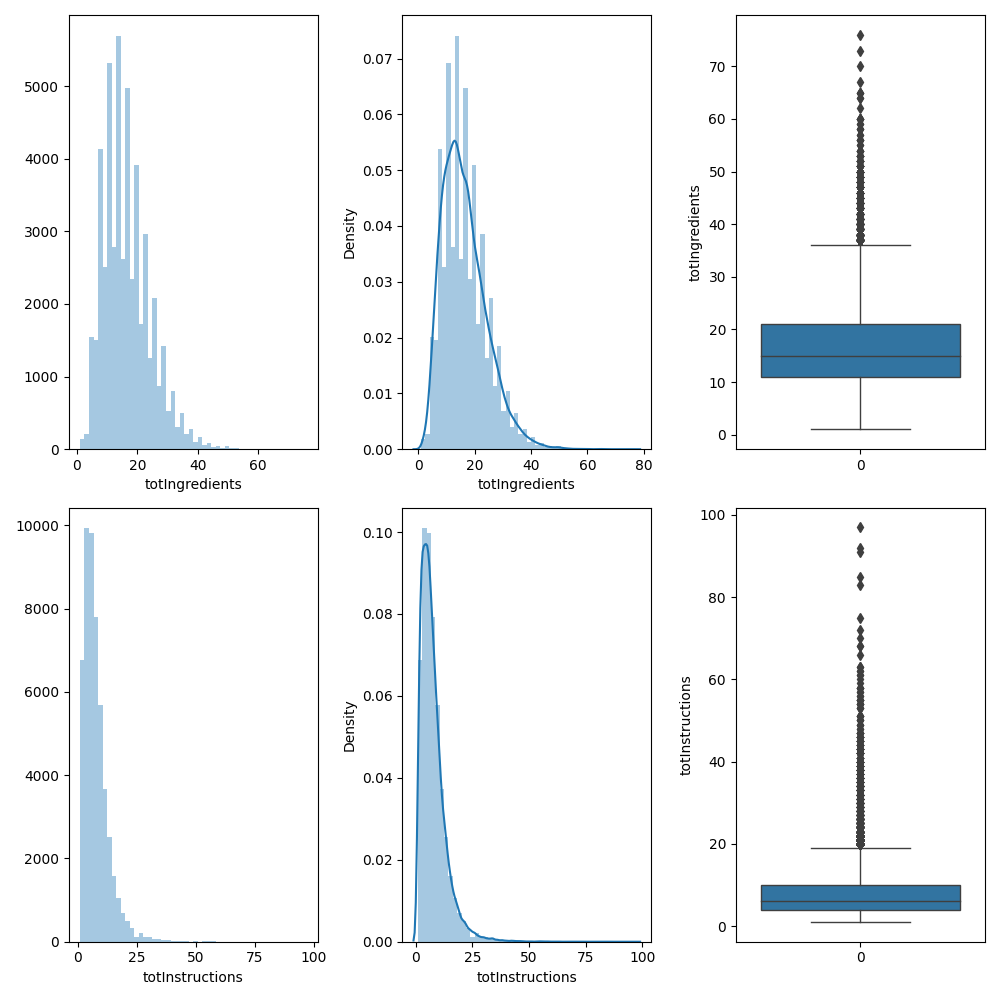
\includegraphics[width =\linewidth]{displot.png}
                \centering
                \caption{Distributions of lines per ingredients and instructions.}
                \label{distributions}
            \end{figure}
        \end{minipage}
    \end{minipage}
    \footnotetext[1]{\tiny J.Marin, A.Biswas, F.Ofli, N.Hynes, A.Salvador, Y.Aytar, I.Weber and A.Torralba, "Recipe1M+: A Dataset for Learning Cross-Modal Embeddings for Cooking Recipes and Food Images", IEEE Trans. Pattern Anal. Mach. Intell., 2019}
\end{frame}

\begin{frame}{RANKING GENERATION}
    The first step is based on choosing a random query, which resembles the title of one of the existing recipes. Subsequently, thanks to the combination of the tf-idf method and the cosine similarity metric, it is possible to generate the first ranking of documents ordered according to relevance with the query. The threshold chosen, for the selection of the most relevant documents, will correspond to the weight assigned by the tf-idf to the target document.
    \begin{minipage}{\linewidth}
        \centering
        \begin{minipage}{0.45\linewidth}
            \begin{block}{\centering tf-idf}
                \small $$ TfIdf(q_t,d) = tf_{q_t,d} \log\frac{N}{df_{q_t}}$$
            \end{block}
        \end{minipage}
        \hspace{0.05\linewidth}
        \begin{minipage}{0.45\linewidth}
            \begin{block}{\centering Cosine similarity}
                \small $$ cosine(q,d) = \frac{\sum_{i=1}^Nqd_i}{\sqrt{\sum_{i=1}^Nq^2}\sqrt{\sum_{i=1}^Nd_i^2}} $$
            \end{block}
        \end{minipage}
    \end{minipage}
\end{frame}

\begin{frame}{RANKING EVALUATION}
    
\end{frame}

\begin{frame}{LANGUAGE MODELS}
    
\end{frame}

\begin{frame}{SMOOTHING METHODS}
    
\end{frame}

\begin{frame}{CORE}
    
\end{frame}

\begin{frame}{TERM-TERM MATRIX}
    
\end{frame}

\begin{frame}{POSITIVE POINTWISE MUTUAL INFORMATIONS (PPMI)}
    
\end{frame}

\begin{frame}{SINGULAR VALUE DECOMPOSITION (SVD)}
    
\end{frame}

\begin{frame}{QUERY EXPANSION}
    
\end{frame}

\begin{frame}{PERPLEXITY}
    
\end{frame}

\begin{frame}{SYSTEM EVALUATION WITH DIFFERENT PARSERS}
    
\end{frame}

\begin{frame}{CONCLUSIONS}
    
\end{frame}







